\section{Cloud Computing}
\label{fundamentals:cloud}

Cloud computing emerged in recent years as an alternative to traditional IT.
Compared to traditional IT, it offers customers far more flexibility in terms of short term access to and scalability of resources, such as servers, databases, communication services, etc.
This increased flexibility is the result of a combination of certain technologies and business models that, although having been around for a while individually, where combined only in recent years.
Since cloud computing is a relatively new phenomenon, there are many definitions of it scattered around. \citeauthor*{cloud:def:towards} looked at over 20 of them and proposed the following definition:

\begin{quote}
	"Clouds are a large pool of easily usable and accessible virtualized resources (such as hardware, development platforms and/or services). These resources can be dynamically reconfigured to adjust to a variable load (scale), allowing also for an optimum resource utilization. This pool of resources is typically exploited by a pay-per-use model in which guarantees are offered by the Infrastructure Provider by means of customized SLAs."\footnote{\nom{Service Level Agreement}{SLA}: "An agreement that sets the expectations between the service provider and the customer and describes the products or services to be delivered, the single point of contact for end-user problems and the metrics by which the effectiveness of the process is monitored and approved."~\autocite{def:sla}}~\autocite{cloud:def:towards}
\end{quote}

The \nom{National Institute of Standards and Technology}{NIST} also proposes a definition:

\begin{quote}
	"Cloud computing is a model for enabling ubiquitous, convenient, on-demand network access to a shared pool of configurable computing resources (e.g., networks, servers, storage, applications, and services) that can be rapidly provisioned and released with minimal management effort or service provider interaction."~\autocite{cloud:def:nist}
\end{quote}

Cloud services can be categorized into different cloud service models, according to what exactly each service encompasses~\autocite{cloudtaxonomy}.
\autoref{image:service_models} shows the three most common service models.
\nom{Infrastructure as a Service}{IaaS} is at the lowest level and provides a customer with access to a virtualization environment on top of servers, storage, and networking. Here, the customer has to manage the \nom{Operating System}{OS}, middleware stack, applications, and data him self.
\nom{Platform as a Service}{PaaS} is the next higher tier, which offers a customer access to a fully managed runtime environment in the cloud.
Here, the customer only has to manage the application they want to execute in the runtime environment and the data.
Finally, \nom{Software as a Service}{SaaS} offers a customer access to a fully managed application running in the cloud.
In this case, the user has to manage neither the OS, nor any middleware, application, or data.

\begin{figure}[!htbp]
	\centering
	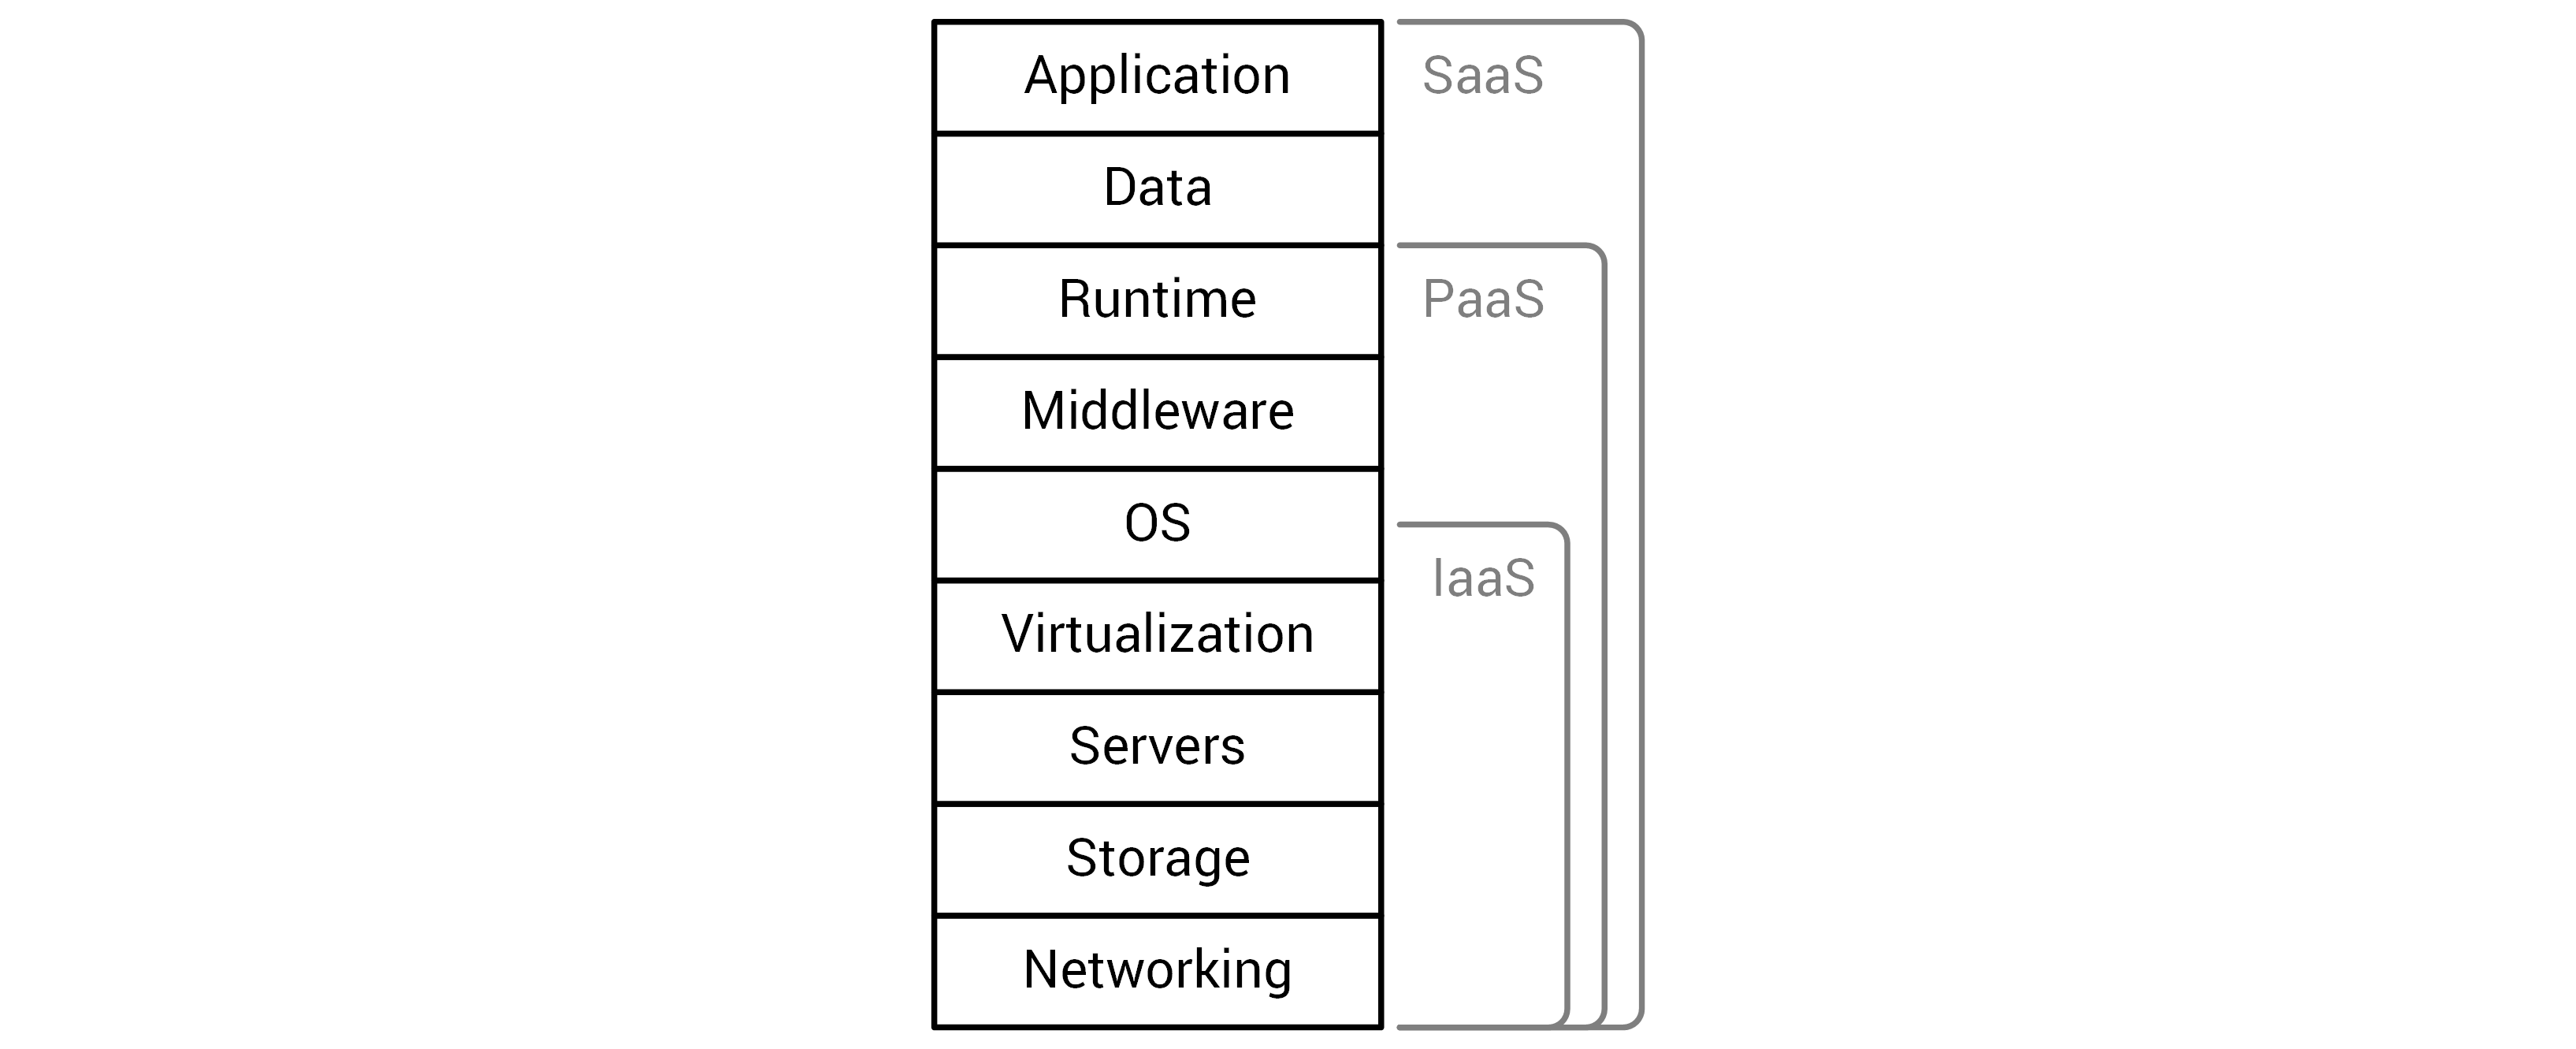
\includegraphics[resolution=600]{fundamentals/assets/service_models}
	\caption{Cloud service models~\autocite[based on][]{cloud:def:gabler}.}
	\label{image:service_models}
\end{figure}

Today, there are many different cloud providers offering a huge selection of services.
The range of providers spans from large corporations like Amazon\footnote{\url{http://aws.amazon.com}\label{aws}}, Google\footnote{\url{https://cloud.google.com}}, Microsoft\footnote{\url{http://azure.microsoft.com}}, and IBM\footnote{\url{http://www.ibm.com/cloud-computing}} to small, focused providers like Heroku\footnote{\url{https://www.heroku.com}} or Jelastic\footnote{\url{http://jelastic.com}} and even solutions to build own clouds, like OpenStack\footnote{\url{https://www.openstack.org}}.
The next section describes Amazon's cloud services in more detail, since those will be used in this diploma thesis.

\subsection{Amazon Web Services}

In 2006, Amazon started offering cloud resource under the umbrella of \nom{Amazon Web Services}{AWS}\footref{aws}.
Since then, their offerings steadily increased and do now comprise over 20 different products and services for computing, data storage, content delivery, analytics, deployment, management, and payment in the cloud.

The most relevant cloud offering for this thesis is \nom{Elastic Compute Cloud}{EC2}\footnote{\url{http://aws.amazon.com/ec2}}, Amazons IaaS offer.
It allows customers to rent virtual server instances at an hourly rate.
These servers are freely configurable, so virtually any software can be installed, making EC2 very versatile.
In addition to general purpose instances (M3), Amazon offers a wide selection of specialized instances, which are optimized for a specific purpose\footnote{\url{http://aws.amazon.com/ec2/instance-types/}}.
These include instances optimized for computation performance (C3), memory-intensive applications (R3), or high storage instances (I2).
For this thesis we will be using Amazons low cost micro instances (T1).

Also of interest to this thesis is Elastic Beanstalk\footnote{\url{http://aws.amazon.com/elasticbeanstalk}}, Amazons PaaS offering.
Customers can upload an application and Elastic Beanstalk takes care of deployment and scaling.
This makes it easier and quicker to use than EC2, but also less flexible.
It could be used instead of a more manual approach with EC2.

Amazon offers multiple ways to interact with cloud resources.
All AWS offerings can be controlled using the AWS Management Console\footnote{\url{http://docs.aws.amazon.com/awsconsolehelpdocs/latest/gsg/getting-started.html}}, a web based management interface that allows customers to start, stop, and manage cloud resources on-demand.
It also provides access to account and billing information.
Additionally, Amazon provides a command line interface, tools for Eclipse and Visual Studio, and \nom{Software Development Kits}{SDKs} for several programming languages, including Java, .Net, Python, Ruby, and the Android and iOS platforms\footnote{\url{https://aws.amazon.com/tools/}}.
In this thesis, we will use the AWS SDK for Java\footnote{\url{https://aws.amazon.com/sdkforjava}} to interact with Amazons cloud resources programmatically.
